\section*{Answer 2}

\subsection*{a)}

\noindent Since $T_A$ and $T_B$ are uniformly distributed
\begin{align*}
  f_{T_A}(t_A) &= \frac{1}{100 - 0} = \frac{1}{100}\\
  f_{T_B}(t_B) &= \frac{1}{100 - 0} = \frac{1}{100}
\end{align*}

Also, since $T_A$ and $T_B$ are indenpendent,
\begin{align*}
  f_{(T_A, T_B)}(t_A, t_B) = f_{T_A}(t_A) f_{T_B}(t_B) = \frac{1}{100} \cdot \frac{1}{100} = \frac{1}{10000} = 10^{-4}
\end{align*}

We found joinst density function. Now we can find joint cdf. Let $u = t_A$, $v = t_B$, then
\begin{align*}
  F_{(X, Y)} (x, y) &= \int_{0}^{y} \int_{0}^{x} f_{(X, Y)} (u, v) du dv\\
  &= \int_{0}^{y} \int_{0}^{x} 10^{-4} du dv\\
  &= \int_{0}^{y} x \cdot 10^{-4} dv\\
  &= xy \cdot 10^{-4}
\end{align*}

\subsection*{b)}

\begin{formula}{}
  In joint cumulative function of two random variables $X$ and $Y$, $F_{(X, Y)} (x, y) = F_X(x) F_Y(y)$ if $X$ and $Y$ are independent. Also, notice that it happened in this question.
  \begin{align*}
      F_{T_A}(t_a) &= \int_{0}^{t_a} f_{T_A}(u)du = t_a \cdot 10^{-2}\\
      F_{T_B}(t_b) &= \int_{0}^{t_b} f_{T_B}(u)du = t_B \cdot 10^{-2}\\
      F_{(T_A, T_B)} (t_A, t_B) &=  F_{T_A}(t_a) \cdot F_{T_B}(t_b) = t_a t_b \cdot 10^{-4}
  \end{align*}
  This fact will be used in the following part.
\end{formula}

We are asked the following probability
\begin{equation*}
  \prob{0 \leq T_A \leq 10,\ 90 \leq T_B \leq 100}
\end{equation*}

We can write it as follows,

\begin{align*}
  \prob{0 \leq T_A \leq 10,\ 90 \leq T_B \leq 100} = F_{(T_A, T_B)} (t_A, t_B) = F_{T_A} (t_a) \cdot F_{T_B} (t_b)
\end{align*}

\subsubsection*{Calculating $F_{T_A} (t_a)$}

\begin{equation*}
  F_{T_A} (t_a) = \int_{0}^{10} f_{T_A} (u) du = \int_{0}^{10} 10^{-2} du = 10^{-2} \cdot 10 = 10^{-1}
\end{equation*}

\subsubsection*{Calculating $F_{T_B} (t_b)$}

\begin{equation*}
  F_{T_B} (t_b) = \int_{90}^{100} f_{T_B} (u) du = \int_{90}^{100} 10^{-2} du = 10^{-2} \cdot 10 = 10^{-1}
\end{equation*}

Then,

\begin{equation*}
  F_{T_A} (t_a) \cdot F_{T_B} (t_b) = 10^{-1} \cdot 10^{-1} = 10^{-2}
\end{equation*}

So the answer is $\dfrac{1}{100}$

\subsection*{c)}

% What is the probability that subject A pushes the button at most 20 seconds after subject B?

% Since it is mentioned that ``at most 20 seconds'', we can think the subject B will push at most in 80 secs and subject A will push. In other words, since $T_A, T_B \in \left[ 0, 100 \right]$, $ 

% We are asked the following
% \begin{align*}
%   \prob{T_B \leq T_A \leq T_B + 20,\ 0 \leq T_B \leq 100}
% \end{align*}

% So,

% \begin{align*}
%   \prob{T_B \leq T_A \leq T_B + 20,\ 0 \leq T_B \leq 100} &= \int_{x}^{y} \int_{0}^{100} f_{(X, Y)} (u, v) du dv\\
%   &= \int_{}^{} \int_{0}^{100} 10^{-2} du dv\\
%   &= \int_{}^{} dv
% \end{align*}

%%%%%%%%%%%%%%%%%%%%%%%%%%%%%%%%%%%

If we think like the way mentioned in the hint. We are asked the ratio of the purple area to all area $\left[ 100 \times 100 \right]$ calculate the probability of the area of the Figure 1. The area is the following
\begin{equation*}
  \prob{(T_A - T_B \leq 20) \cap (T_B \leq T_A)}
\end{equation*}

\begin{figure}[ht!]
  \centering
  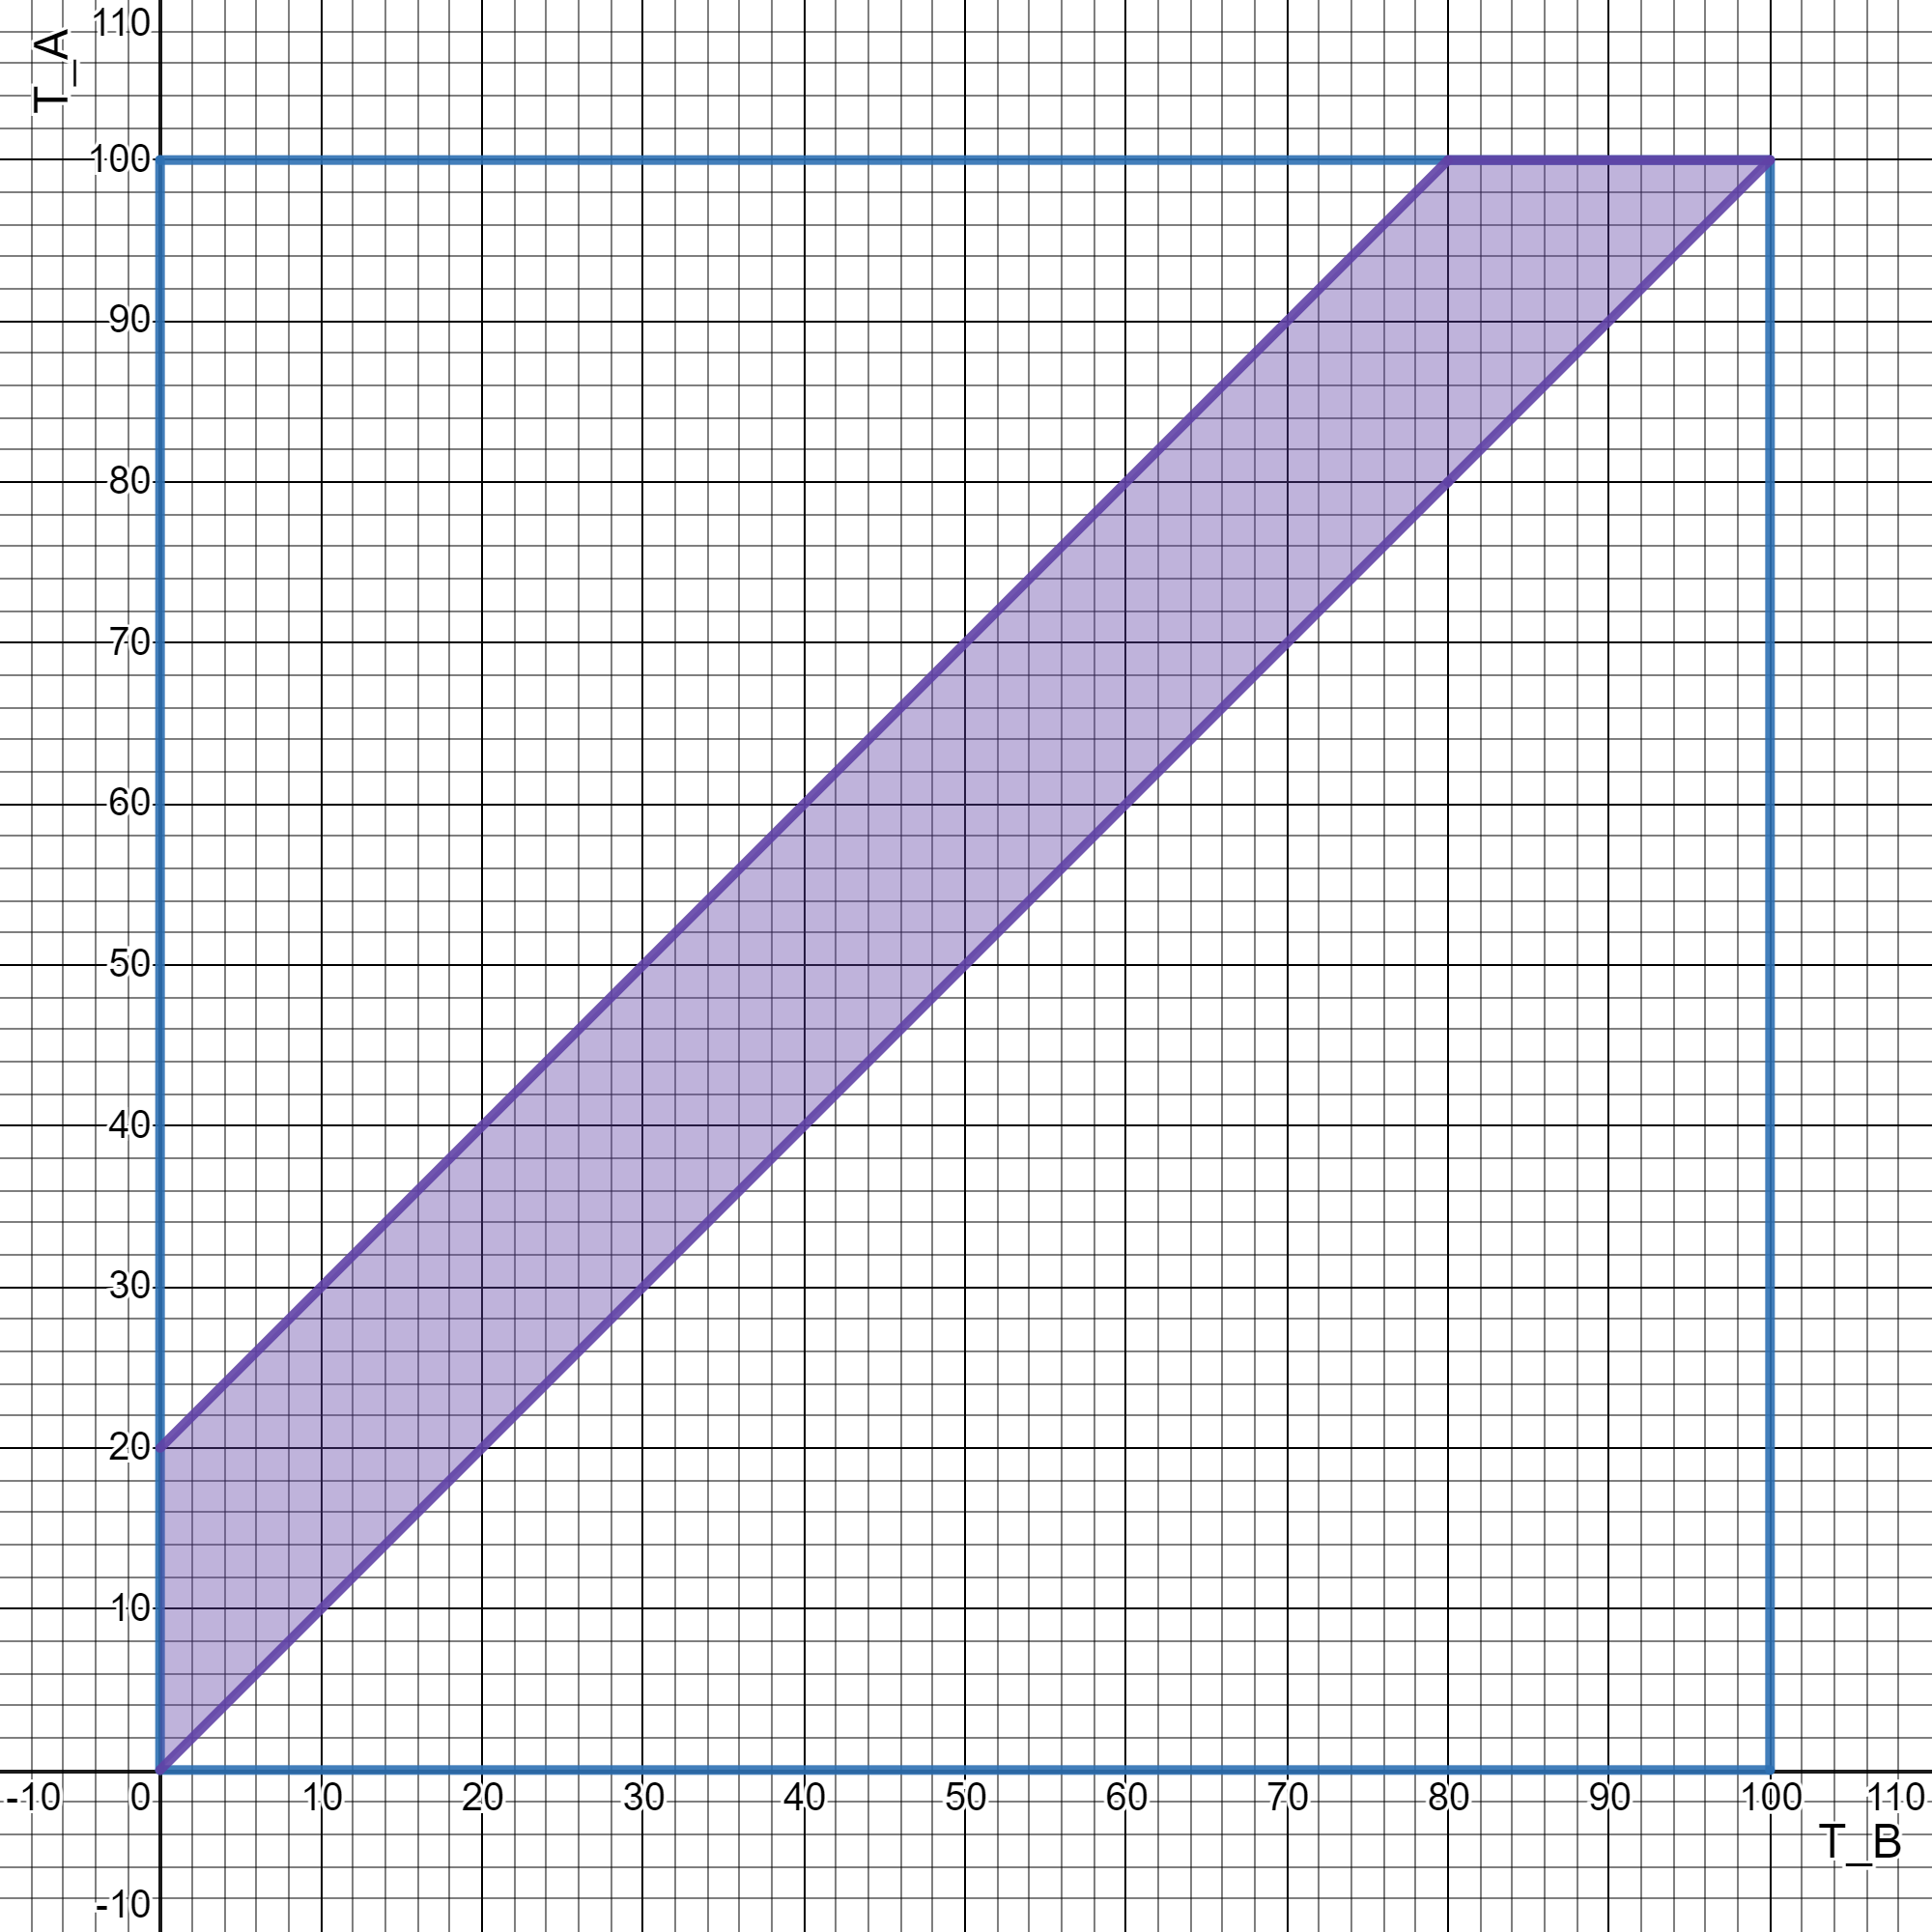
\includegraphics[width=.4\textwidth]{img/q2-c.png}
  \caption{}
\end{figure}

\begin{multicols}{2}
\begin{itemize}
  \item $\textnormal{The area of purple part} = 1800$
  \item $\textnormal{The area of the whole part} = 10^4$
\end{itemize}
\end{multicols}

So, the ratio of the purple area to whole area is the answer and it is $\dfrac{18}{100} = 0.18$.

\newpage
\subsection*{d)}

Again, if we think like the way mentioned in the hint. We are asked the ratio of the purple area to all area $\left[ 100 \times 100 \right]$ calculate the probability of the area of the Figure 2. The area is the following
\begin{equation*}
  \prob{(|T_A - T_B| \leq 30)}
\end{equation*}

\begin{figure}[ht!]
  \centering
  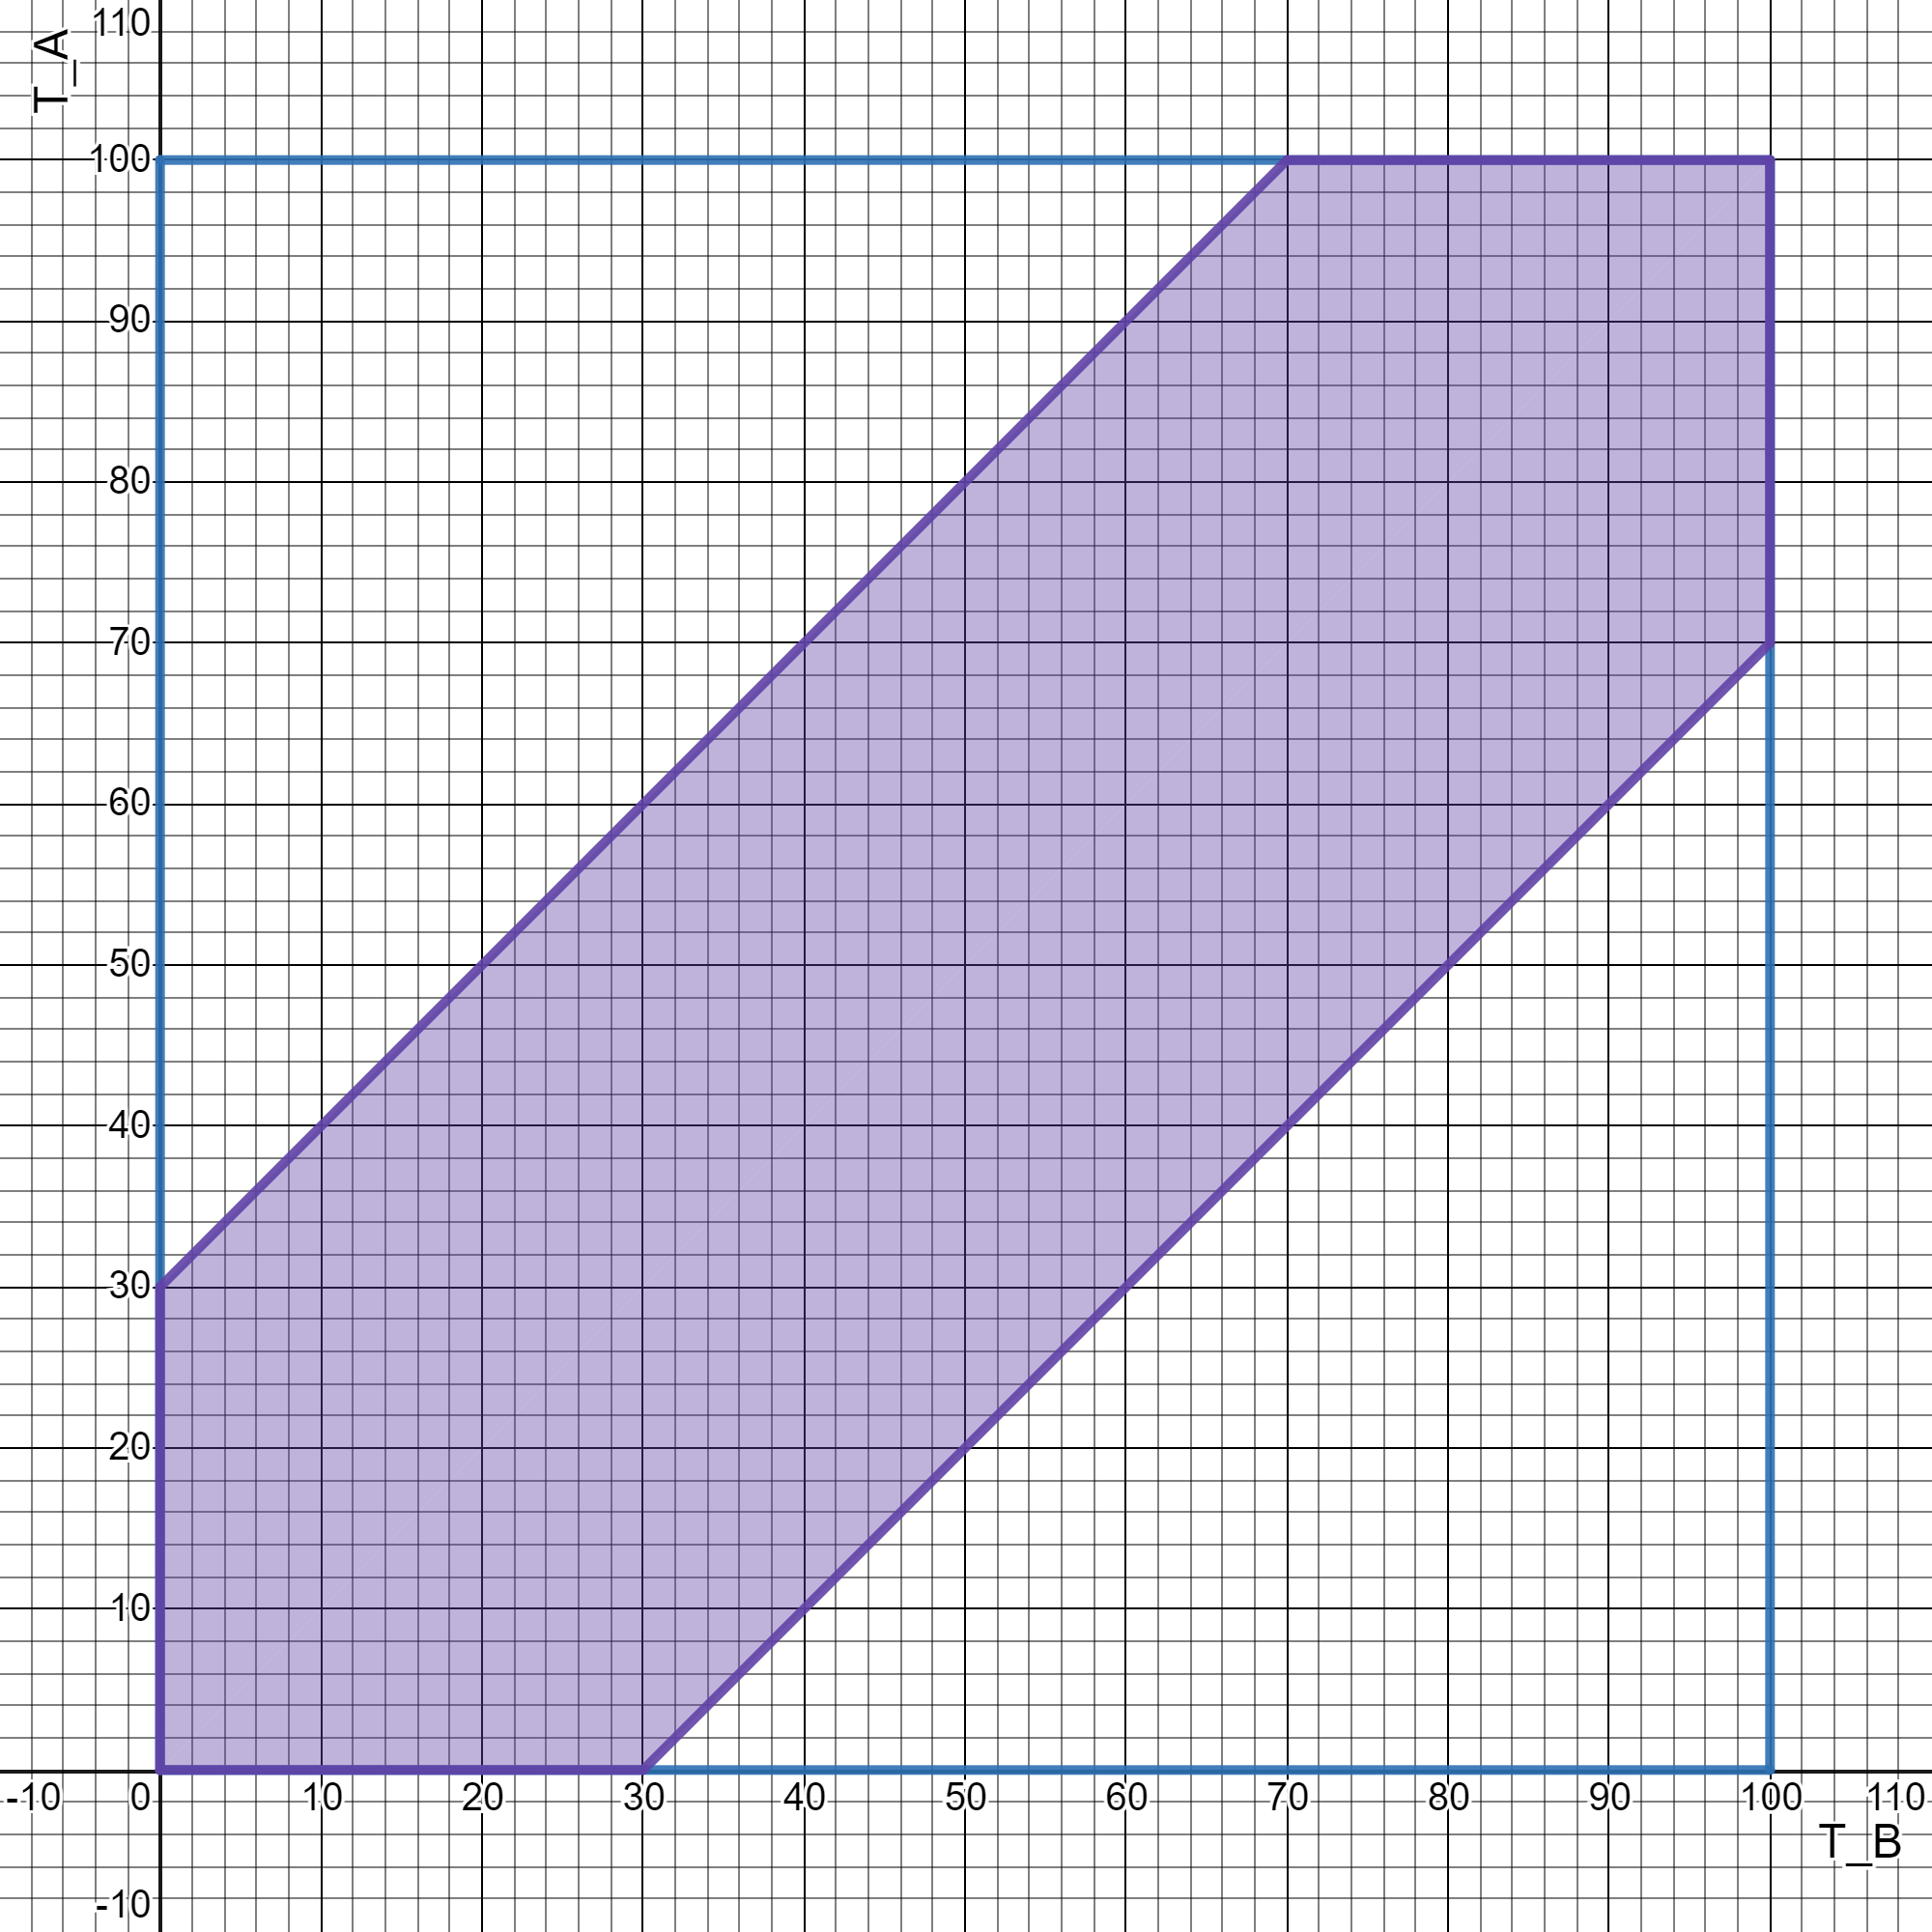
\includegraphics[width=.5\textwidth]{img/q2-d.png}
  \caption{}
\end{figure}

\begin{multicols}{2}
  \begin{itemize}
    \item $\textnormal{The area of purple part} = 5100$
    \item $\textnormal{The area of the whole part} = 10^4$
  \end{itemize}
\end{multicols}

So, the ratio of the purple area to whole area is the answer and it is $\dfrac{51}{100} = 0.51$.
